\documentclass{article}
\usepackage[T1]{fontenc}
\usepackage{lmodern}
\usepackage{graphicx}
\usepackage{amsmath,amssymb}
\usepackage[a4paper,margin=2cm]{geometry}
\usepackage[absolute,overlay]{textpos}
\setlength{\TPHorizModule}{1mm}
\setlength{\TPVertModule}{1mm}
\usepackage[indonesian]{babel}
\usepackage{hyperref}
\setlength{\emergencystretch}{2em}
% unit: Halaman 5

\begin{document}

% === Halaman 5 (python/native) ===

5

• Salah satu metrik penting di dalam teori informasi adalah entropi. 

• Entropi mengukur ketidakpastian atau jumlah rata-rata informasi di dalam 

pesan.

• Semakin acak suatu data, semakin tinggi entropinya. Cipherteks adalah 

pesan dengan entropi yang tinggi.

• Entropi biasanya dinyatakan dalam satuan bit.

• Secara umum, entropi pesan X dihitung dengan rumus:



X = variabel acak yang menyatakan pesan


xi = simbol ke-i di dalam pesan

            n = banyak simbol di dalam pesan


p(xi) = peluang kemunculan xi

% deskripsi: gambar native xref 41
\noindent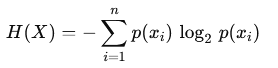
\includegraphics[width=0.85\textwidth]{../../images/python/page_005_img_01.png}

\end{document}
